% Created by tikzDevice version 0.12.3.1 on 2022-09-02 16:26:29
% !TEX encoding = UTF-8 Unicode
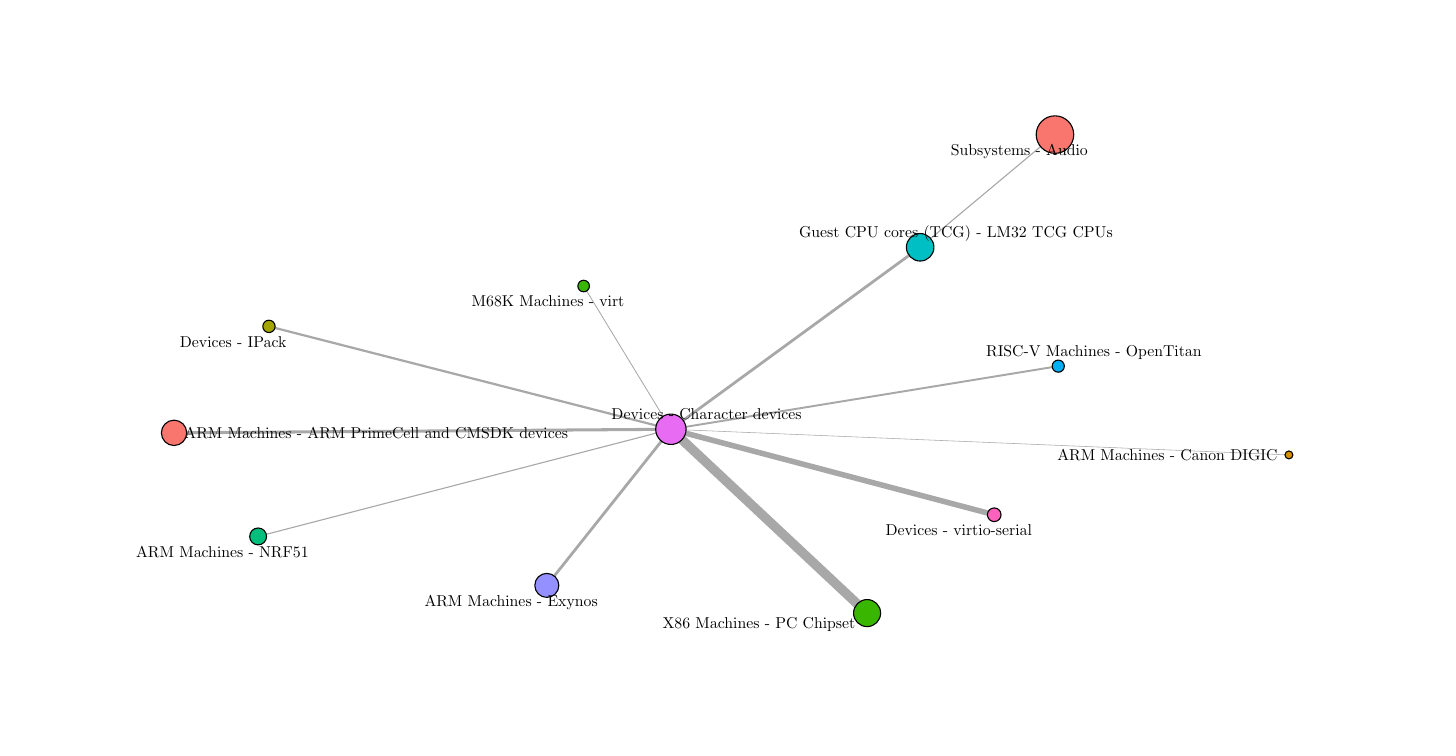
\begin{tikzpicture}[x=1pt,y=1pt]
\definecolor{fillColor}{RGB}{255,255,255}
\path[use as bounding box,fill=fillColor,fill opacity=0.00] (0,0) rectangle (505.89,252.94);
\begin{scope}
\path[clip] (  0.00,  0.00) rectangle (505.89,252.94);
\definecolor{fillColor}{RGB}{255,255,255}

\path[fill=fillColor] (  0.00,  0.00) rectangle (505.89,252.94);
\end{scope}
\begin{scope}
\path[clip] ( 32.75, 32.75) rectangle (475.89,222.94);
\definecolor{drawColor}{gray}{0.66}

\path[draw=drawColor,line width= 1.1pt,line join=round] ( 52.89,106.53) -- (232.43,107.82);

\path[draw=drawColor,line width= 0.2pt,line join=round] (455.75, 98.55) -- (232.43,107.82);

\path[draw=drawColor,line width= 1.0pt,line join=round] (187.59, 51.41) -- (232.43,107.82);

\path[draw=drawColor,line width= 0.4pt,line join=round] ( 83.27, 69.10) -- (232.43,107.82);

\path[draw=drawColor,line width= 0.8pt,line join=round] (232.43,107.82) -- ( 87.19,145.00);

\path[draw=drawColor,line width= 2.0pt,line join=round] (232.43,107.82) -- (349.26, 76.93);

\path[draw=drawColor,line width= 1.0pt,line join=round] (232.43,107.82) -- (322.50,173.58);

\path[draw=drawColor,line width= 0.3pt,line join=round] (232.43,107.82) -- (200.90,159.58);

\path[draw=drawColor,line width= 0.7pt,line join=round] (232.43,107.82) -- (372.40,130.63);

\path[draw=drawColor,line width= 3.4pt,line join=round] (232.43,107.82) -- (303.32, 41.40);

\path[draw=drawColor,line width= 0.4pt,line join=round] (322.50,173.58) -- (371.21,214.30);
\definecolor{drawColor}{RGB}{0,0,0}
\definecolor{fillColor}{RGB}{248,118,109}

\path[draw=drawColor,line width= 0.4pt,line join=round,line cap=round,fill=fillColor] ( 52.89,106.53) circle (  4.58);
\definecolor{fillColor}{RGB}{216,144,0}

\path[draw=drawColor,line width= 0.4pt,line join=round,line cap=round,fill=fillColor] (455.75, 98.55) circle (  1.43);
\definecolor{fillColor}{RGB}{149,144,255}

\path[draw=drawColor,line width= 0.4pt,line join=round,line cap=round,fill=fillColor] (187.59, 51.41) circle (  4.34);
\definecolor{fillColor}{RGB}{0,191,125}

\path[draw=drawColor,line width= 0.4pt,line join=round,line cap=round,fill=fillColor] ( 83.27, 69.10) circle (  3.05);
\definecolor{fillColor}{RGB}{231,107,243}

\path[draw=drawColor,line width= 0.4pt,line join=round,line cap=round,fill=fillColor] (232.43,107.82) circle (  5.49);
\definecolor{fillColor}{RGB}{163,165,0}

\path[draw=drawColor,line width= 0.4pt,line join=round,line cap=round,fill=fillColor] ( 87.19,145.00) circle (  2.23);
\definecolor{fillColor}{RGB}{255,98,188}

\path[draw=drawColor,line width= 0.4pt,line join=round,line cap=round,fill=fillColor] (349.26, 76.93) circle (  2.46);
\definecolor{fillColor}{RGB}{0,191,196}

\path[draw=drawColor,line width= 0.4pt,line join=round,line cap=round,fill=fillColor] (322.50,173.58) circle (  4.97);
\definecolor{fillColor}{RGB}{57,182,0}

\path[draw=drawColor,line width= 0.4pt,line join=round,line cap=round,fill=fillColor] (200.90,159.58) circle (  2.09);
\definecolor{fillColor}{RGB}{0,176,246}

\path[draw=drawColor,line width= 0.4pt,line join=round,line cap=round,fill=fillColor] (372.40,130.63) circle (  2.19);
\definecolor{fillColor}{RGB}{248,118,109}

\path[draw=drawColor,line width= 0.4pt,line join=round,line cap=round,fill=fillColor] (371.21,214.30) circle (  6.78);
\definecolor{fillColor}{RGB}{57,182,0}

\path[draw=drawColor,line width= 0.4pt,line join=round,line cap=round,fill=fillColor] (303.32, 41.40) circle (  4.89);

\node[text=drawColor,anchor=base,inner sep=0pt, outer sep=0pt, scale=  0.57] at (125.97,104.57) {ARM Machines - ARM PrimeCell and CMSDK devices};

\node[text=drawColor,anchor=base,inner sep=0pt, outer sep=0pt, scale=  0.57] at (411.84, 96.59) {ARM Machines - Canon DIGIC};

\node[text=drawColor,anchor=base,inner sep=0pt, outer sep=0pt, scale=  0.57] at (174.70, 43.92) {ARM Machines - Exynos};

\node[text=drawColor,anchor=base,inner sep=0pt, outer sep=0pt, scale=  0.57] at ( 70.37, 61.62) {ARM Machines - NRF51};

\node[text=drawColor,anchor=base,inner sep=0pt, outer sep=0pt, scale=  0.57] at (245.33,111.40) {Devices - Character devices};

\node[text=drawColor,anchor=base,inner sep=0pt, outer sep=0pt, scale=  0.57] at ( 74.27,137.49) {Devices - IPack};

\node[text=drawColor,anchor=base,inner sep=0pt, outer sep=0pt, scale=  0.57] at (336.45, 69.46) {Devices - virtio-serial};

\node[text=drawColor,anchor=base,inner sep=0pt, outer sep=0pt, scale=  0.57] at (335.41,177.17) {Guest CPU cores (TCG) - LM32 TCG CPUs};

\node[text=drawColor,anchor=base,inner sep=0pt, outer sep=0pt, scale=  0.57] at (188.03,152.10) {M68K Machines - virt};

\node[text=drawColor,anchor=base,inner sep=0pt, outer sep=0pt, scale=  0.57] at (385.28,134.19) {RISC-V Machines - OpenTitan};

\node[text=drawColor,anchor=base,inner sep=0pt, outer sep=0pt, scale=  0.57] at (358.33,206.83) {Subsystems - Audio};

\node[text=drawColor,anchor=base,inner sep=0pt, outer sep=0pt, scale=  0.57] at (264.26, 35.76) {X86 Machines - PC Chipset};
\end{scope}
\end{tikzpicture}
